\section*{Problem 4}

\paragraph{b} With the default shrinkage parameter (0.001) we obtained the following Relative Influence Plot and Partial Dependence Plot: 

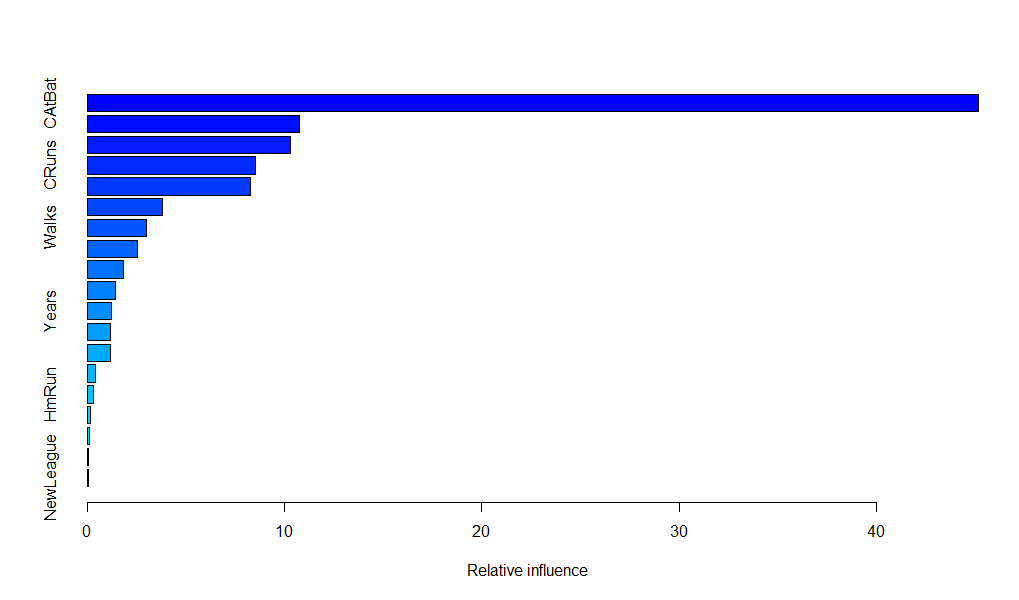
\includegraphics[width=\textwidth]{img/relativeInfluencePlot.png}

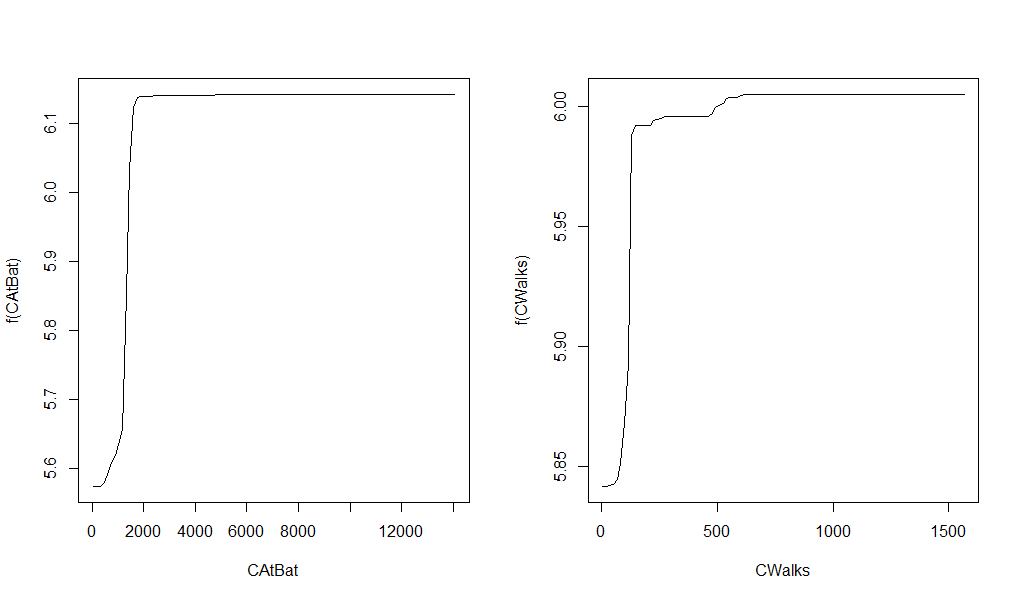
\includegraphics[width=\textwidth]{img/partialDependencePlots.png}

We then execute for a $\delta$ from 0.01 to 1 and plot the train MSE and test MSE: 

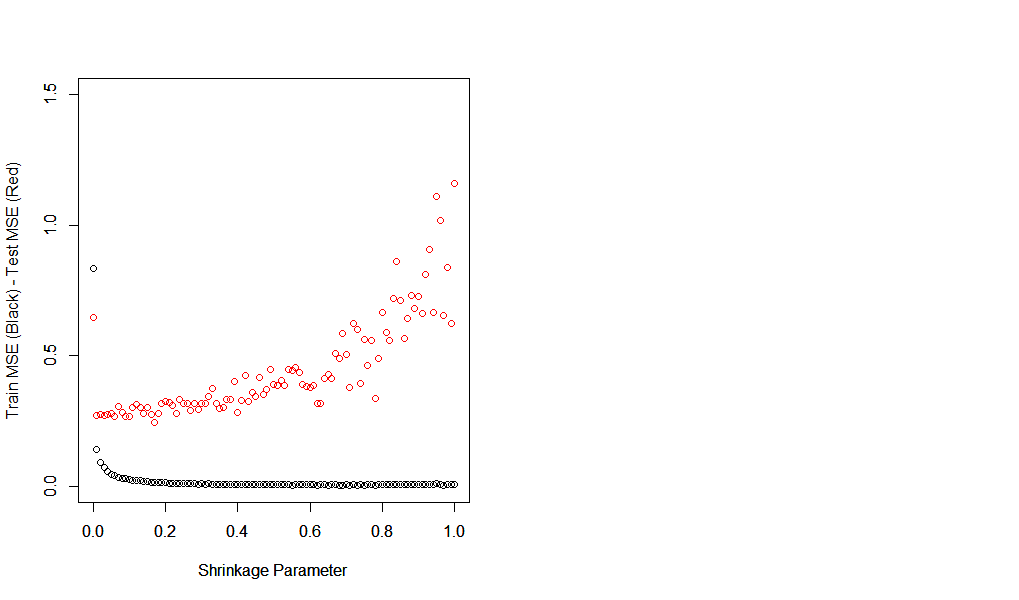
\includegraphics[width=\textwidth]{img/shrkg.png}

We choose $\delta = 0.2 $ 

%TODO justify 0.2.... leverage point ?

\paragraph{c} We have the following values: \\

\begin{tabular}{|c|c|}
	\hline 
	Algorithme & MSE \\ 
	\hline 
	Boosting & \textbf{0.24} \\ 
	\hline 
	Least Squares & 0.49 \\ 
	\hline 
	Ridge & 0.56 \\ 
	\hline 
\end{tabular} 


 
\paragraph{d} Variable importance: \\

For boosting the graphing on point b show the actual following values: \\

\begin{table}[]
	\centering
	\caption{Variable importance for Boosting}
	\label{my-label}
	\begin{tabular}{lllllll}
		var        & rel.inf     &  &  &  &  &  \\
		CAtBat     & 45.18862170 &  &  &  &  &  \\
		CWalks     & 10.76140033 &  &  &  &  &  \\
		CHits      & 10.27594487 &  &  &  &  &  \\
		CRuns      & 8.49553266  &  &  &  &  &  \\
		CRBI       & 8.27788387  &  &  &  &  &  \\
		AtBat      & 3.77926831  &  &  &  &  &  \\
		Walks      & 2.97904456  &  &  &  &  &  \\
		CHmRun     & 2.50711182  &  &  &  &  &  \\
		Hits       & 1.81700963  &  &  &  &  &  \\
		RBI        & 1.39305145  &  &  &  &  &  \\
		Years      & 1.18646093  &  &  &  &  &  \\
		PutOuts    & 1.18241928  &  &  &  &  &  \\
		Runs       & 1.15779063  &  &  &  &  &  \\
		Assists    & 0.38518856  &  &  &  &  &  \\
		HmRun      & 0.29914573  &  &  &  &  &  \\
		Errors     & 0.15584311  &  &  &  &  &  \\
		Division   & 0.07288507  &  &  &  &  &  \\
		League     & 0.04818061  &  &  &  &  &  \\
		New League & 0.03721686  &  &  &  &  & 
	\end{tabular}
\end{table}

For Ridge: \\




For linear regression, the two highest coefficient are AtBat and Hits

